\documentclass[superscriptaddress,aps,prb,11pt]{revtex4-1}
\draft

\usepackage{amsmath}
\usepackage{graphicx}
\usepackage{color}
\usepackage{subfigure}
\usepackage{hyperref}

\begin{document}

\title{Experimental Search for Lorentz Violation in Antihydrogen}
\author{F. Isono}
\affiliation{Department of Physics, University of California, Berkeley, CA 94720-7300, USA}
\affiliation{Department of Physics, Tokyo Institute of Technology, Meguro, Tokyo 152-8551, Japan}

\author{Z. Vendeiro}
\affiliation{Department of Physics, University of California, Berkeley, CA 94720-7300, USA}

\author{J. Fajans}
\affiliation{Department of Physics, University of California, Berkeley, CA 94720-7300, USA}
\affiliation{Lawrence Berkeley National Laboratory, Berkeley, CA 94720, USA}

\author{A. Charman}
\affiliation{Department of Physics, University of California, Berkeley, CA 94720-7300, USA}
\affiliation{Lawrence Berkeley National Laboratory, Berkeley, CA 94720, USA}

\author{M. Reinsch}
\affiliation{Department of Physics, University of California, Berkeley, CA 94720-7300, USA}
\affiliation{Lawrence Berkeley National Laboratory, Berkeley, CA 94720, USA}

\author{J. S. Wurtele}
\affiliation{Department of Physics, University of California, Berkeley, CA 94720-7300, USA}
\affiliation{Lawrence Berkeley National Laboratory, Berkeley, CA 94720, USA}

\author{A. Lotta-Folks}

\begin{abstract}
Data on locations of antihydrogen annihilations in the ALPHA trap is retrospectively annalyzed for temporal variation due to violations of Lorentz Invariance as the Earth rotates and orbits the sun.  To be continued\ldots
\end{abstract}

\maketitle

General relativity purports that a particle's charge is independent of the observer's reference frame.  Although the theoretical underpinnings of this prediction are strong, experimental verification of fundamental predictions of physics are critical to assessing the axioms necessary to develop such theory.  In this spirit, we have performed a retrospective analysis on the data collected during the ALPHA experiment's runs in 2010 and 2011 to examine it for indications of Lorentz violation in the antimatter sector.

Proposed violations are expected to be correlated with the velocity and/or orientation of the trap relative to a preferred frame.  As is standard in searches for Lorentz violation, speed is measured relative to the rest frame of the CMB.

\begin{figure}
  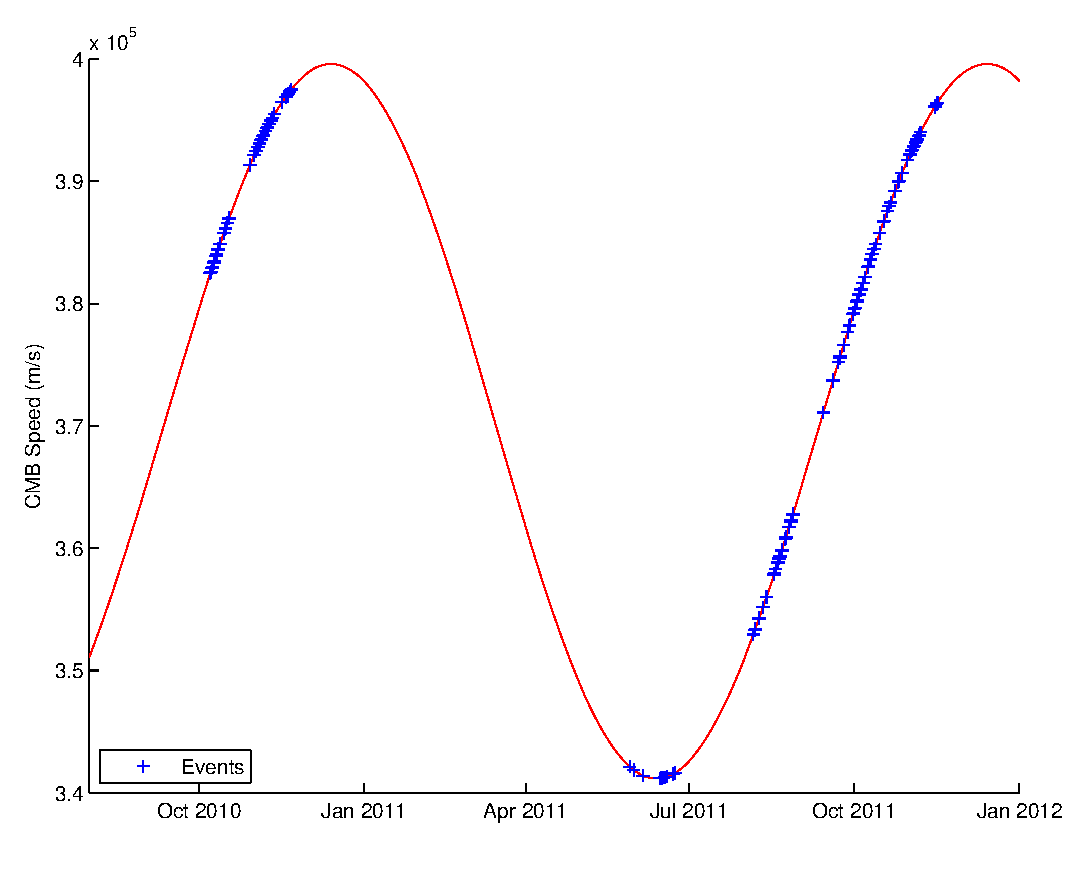
\includegraphics[scale=0.3]{True_Event_Distribution.eps}
  \label{fig:true_event_distribution}
  \caption{The CMB speed of the Earth over the period of time during which ALPHA was running.  Times of the various $\bar{H}$ annihilations events are marked.}
\end{figure}

\section{Methods Summary}
A bound on the temporal variation of the antihydrogen charge is performed by comparison of a test statistic $S$, constructed to approximate the magnitude of a Fourier coefficient, of the collected data to simulated distributions of this statistic.  A statistically significant nonzero value of $S$ would indicate a violation of Lorentz Invariance.

Define $f(t)$ to be a function that maps times of $\bar{H}$ annihilations to the $z$ position of those annihilations.

\begin{figure}
  \centering
  \subfigure[\ Full Domain of CDF]{
  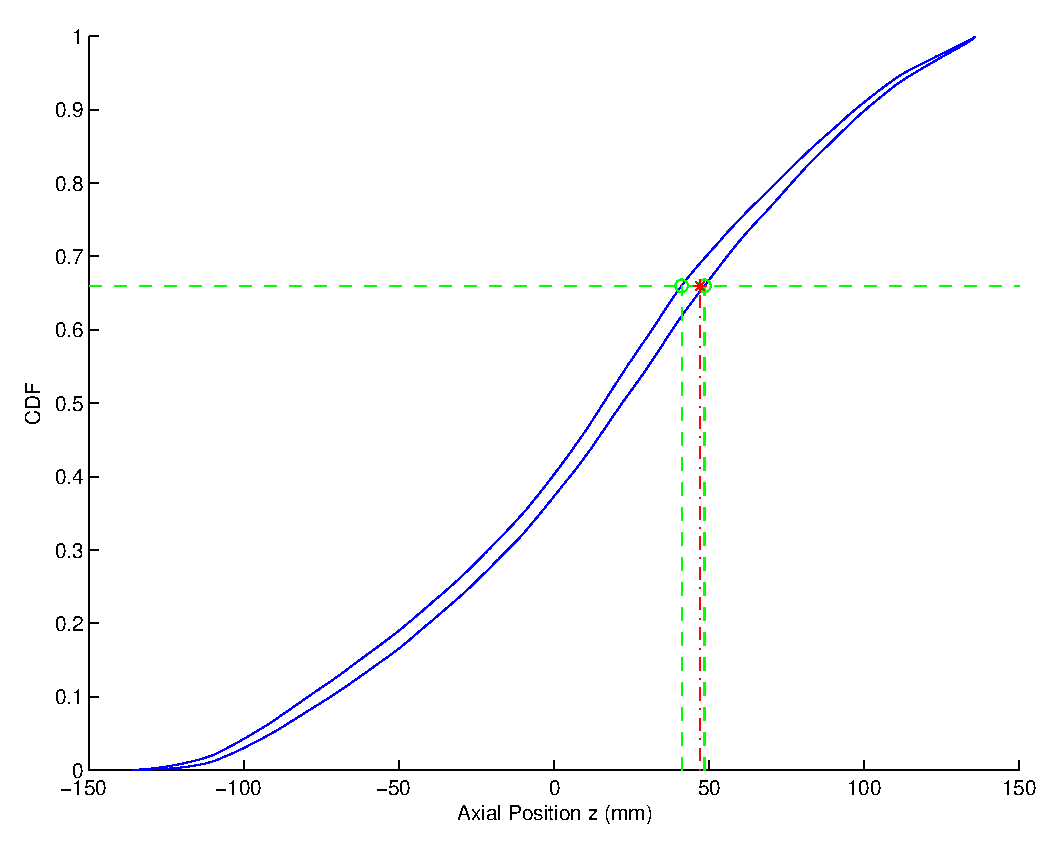
\includegraphics[scale=0.3]{CDF_Interpolation_Plot1.eps}}
  \subfigure[\ Region of Interest]{
  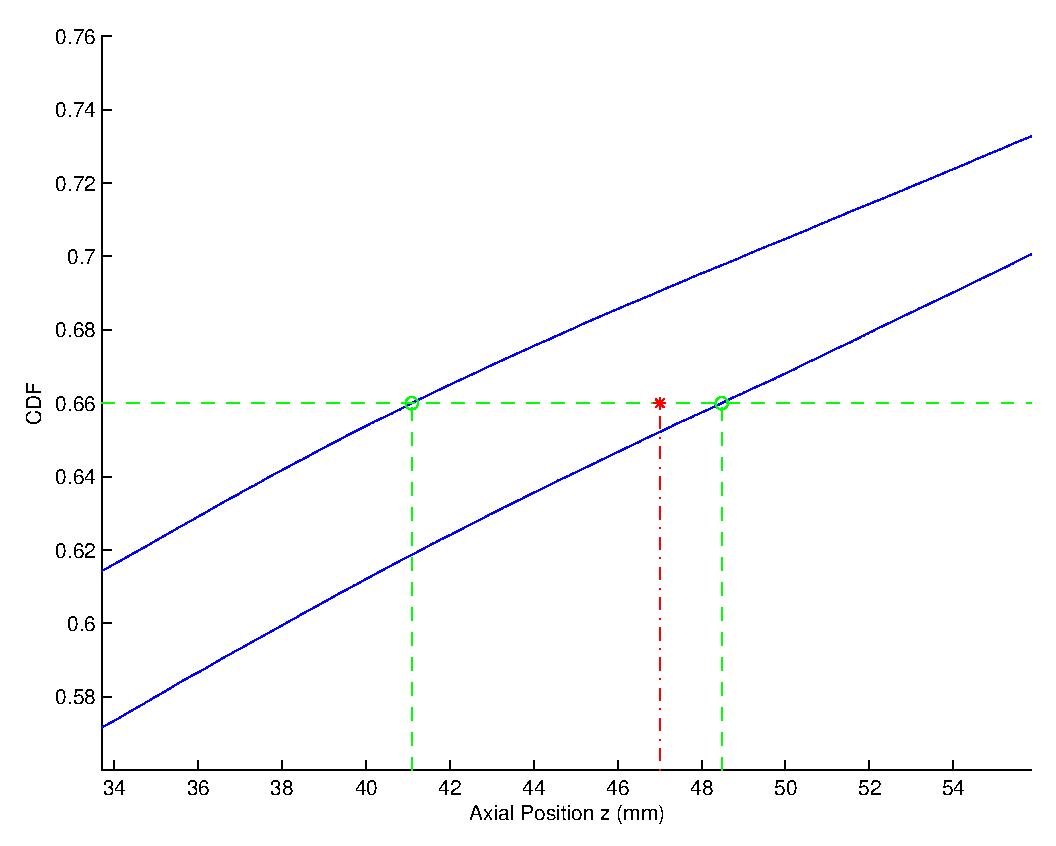
\includegraphics[scale=0.3]{CDF_Interpolation_Plot2.eps}}
  \label{fig:z_interpolation}
  \caption{Graphical depiction of the annihilation $z$ value selection algorithm.  An empirical CDF is generated for several different charges.  Two of such CDFs are shown with linear interpolation (blue solid curves).  When a $z$ position is desired for a given charge, a random value, here shown as 0.66, is picked and the values of the inverse CDFs, which can be read off of the $x$-axis here, are determined (green dashed lines).  The weighted average is then taken to give the $z$ value for the desired charge (red dash-dot line).  Here the charge is closer in value to the charge giving the right CDF than the left CDF.}
\end{figure}

\subsection*{Time Selection}
I dunno, ask Fumika how we do this.


\subsection*{Position Selection}
Creation of pseudo-data sets requires an algorithm capable of generating $z$ positions of $\bar{H}$ annihilations for arbitrary charge values.  This is achieved by randomly sampling an approximated inverse CDF of the annihilation locations along the trap axis for the given charge.

Using the symplectic integrator discussed in Ref. \onlinecite{fractionalcharge}, a list of annihilation $z$ coordinates is created for both quip directions for several different charges.  These lists are then adjusted to account for effects from detector smearing and missed detections due to cosmic ray filtering criteria, also discussed in Ref. \onlinecite{fractionalcharge}.  This provides empirical CDFs of simulated annihilations for various charges.  A simulated $z$ value for these charges can be chosen by selecting a random value from a uniform distribution on the interval (0,1), then determining the associated $z$ value by linearly interpolating the inverse CDF.  For charges between the discrete list of values for which the symplectic integrator has provided results, $z$ positions can be assigned by performing the above interpolation on the two neighboring empirical CDFs using the same random value, then further interpolating by taking a weighted average of the two results.  The weights are chosen to provide a linear interpolation between the two sampled charge distributions.  The process is summarized in Fig. \ref{fig:z_interpolation}.

\begin{acknowledgments}
To be continued\ldots
\end{acknowledgments}

\section{Notes}
The graphs right now are created in Matlab.  In the future they will be made in Origin and should look prettier.

We also need to add the other authors and stuff to the fractional charge paper, but I'm waiting to see if I can find an automatically-generated bibtex entry somewhere.

Is that the proper address for Tokyo Institute of technology?

The reference to the figure at the end of the Position Selection subsection is correct in the source, but the output pdf points to Fig 1 instead.  This will likely resolve itself once a reference to the first figure is added.

\nocite{fractionalcharge}
\bibliographystyle{plain}
\bibliography{References.bib}

\end{document}